\documentclass[journal=jpcbfk]{achemso}

\usepackage[version=3]{mhchem}
\usepackage[T1]{fontenc}
\newcommand*\mycommand[1]{\texttt{\emph{#1}}}
\newcommand{\todo}[1]{\textcolor{red}{#1}}

\usepackage{rotating}
\usepackage{upgreek}				
\usepackage{xcolor}
\usepackage{booktabs}
\usepackage{multirow}
\usepackage{lmodern}
\usepackage{microtype}
\usepackage{xr}
\externaldocument{manuscriptPGPE}
\usepackage{soul} % for highlights with \hl{} 

\author{O. H. Samuli Ollila}
\email{samuli.ollila@helsinki.fi}
%\homepage[]{Your web page}
\affiliation{Institute of Organic Chemistry and Biochemistry,
Academy of Sciences of the Czech Republic, 
Prague 6, Czech Republic}
\affiliation{Institute of Biotechnology, University of Helsinki}


\SectionNumbersOn

\renewcommand{\thetable}{S\arabic{table}}%
\renewcommand{\thefigure}{S\arabic{figure}}%
\renewcommand{\thesection}{S\arabic{section}}%
\renewcommand{\thepage}{S\arabic{page}}%

\title{ Supporting Information:\\ NMRlipids IV: Headgroup \& glycerol backbone structures, and cation binding in bilayers with PE and PG lipids }

\begin{document}

\newpage
%\tableofcontents

\section{Simulated systems}

\subsection{CHARMM36}

{\it POPC:POPE mixtures} Data is available at \cite{POPCcharmm300K,POPC1POPE1charmm36}.
300 K with v-rescale (tau=0.1 ps),
1 bar with PR semiisotropic (tau=4 ps, compressibility=4.5e-5 bar$^{-1}$),
PME order 4 and space 0.12,
rcoulomb and rvdw 1.0,
128 lipids per leaflet,
no ion \todo{Full simulation details by Fuchs et al.}

{\it POPC:POPG mixture with additional calcium} \todo{Simulation details by J. Madsen.}

\subsection{CHARMM36ua}

{\it POPE} Data is available at \cite{charmm36uaPOPEfiles}. \todo{Simulation details by  T. Piggot.}

%\subsection{MacRog}

%\subsection{Lipid17}

\subsection{Slipids}
{\it POPE} Data is available at \cite{slipidsPOPEfiles}. \todo{Simulation details by  T. Piggot.}

{\it DPPE} Data is available at \cite{slipidsDPPEfiles}. \todo{Simulation details by F. Favela.}

{\it POPG} Data is available at \cite{slipidsPOPGfiles}. \todo{Simulation details by F. Favela.}

{\it DPPG} Data in 298~K is available at \cite{slipidsDPPGfilesT298K} and in 314~K at \cite{slipidsDPPGfiles}.  \todo{Simulation details by F. Favela.}

\subsection{Berger}

{\it POPE} Data is available at \cite{bergerPOPEfiles,berger2POPEfiles}. \todo{Simulation details by  T. Piggot.}

{\it DOPE} Data is available at \cite{bergerDOPEfiles,berger2DOPEfiles}. \todo{Simulation details by  T. Piggot.}

{\it POPC:POPE, POPC:DOPE and DOPC:DOPE mixtures} Data is available at \cite{POPCberger300K,POPC1POPE1berger}. 
300 K with v-rescale (tau=0.1 ps),
1 bar with PR semiisotropic (tau=4 ps, compressibility=4.5e-5 bar$^{-1}$),
PME order 4 and space 0.12,
rcoulomb and rvdw 1.0,
128 lipids per leaflet,
no ion \todo{Simulation details by Fuchs et al.}

\subsection{GROMOS 43A1-S3}

{\it POPE} Data is available at \cite{gromos43a1s3POPEfiles}. \todo{Simulation details by  T. Piggot.}

\subsection{OPLS-UA}

{\it POPE} Data is available at \cite{OPLSuaPOPEfiles}. \todo{Simulation details by  T. Piggot.}

{\it POPE with vdW interaction in H} Data is available at \cite{OPLSuaWvdWPOPEfiles}. \todo{Simulation details by  T. Piggot.}

\subsection{GROMOS-CKP and GROMOS-CKPM}

{\it POPE} Data is available at \cite{gromosCKPpope}. \todo{Simulation details by  T. Piggot.}

{\it DOPE} Data is available at \cite{gromosCKPdope}. \todo{Simulation details by  T. Piggot.}

{\it DPPE} Data is available at \cite{gromosCKPdppe}. \todo{Simulation details by  T. Piggot.}

\clearpage
\section{R-PDLF and SDROSS experiments}

\begin{figure}[]
%  \centering
  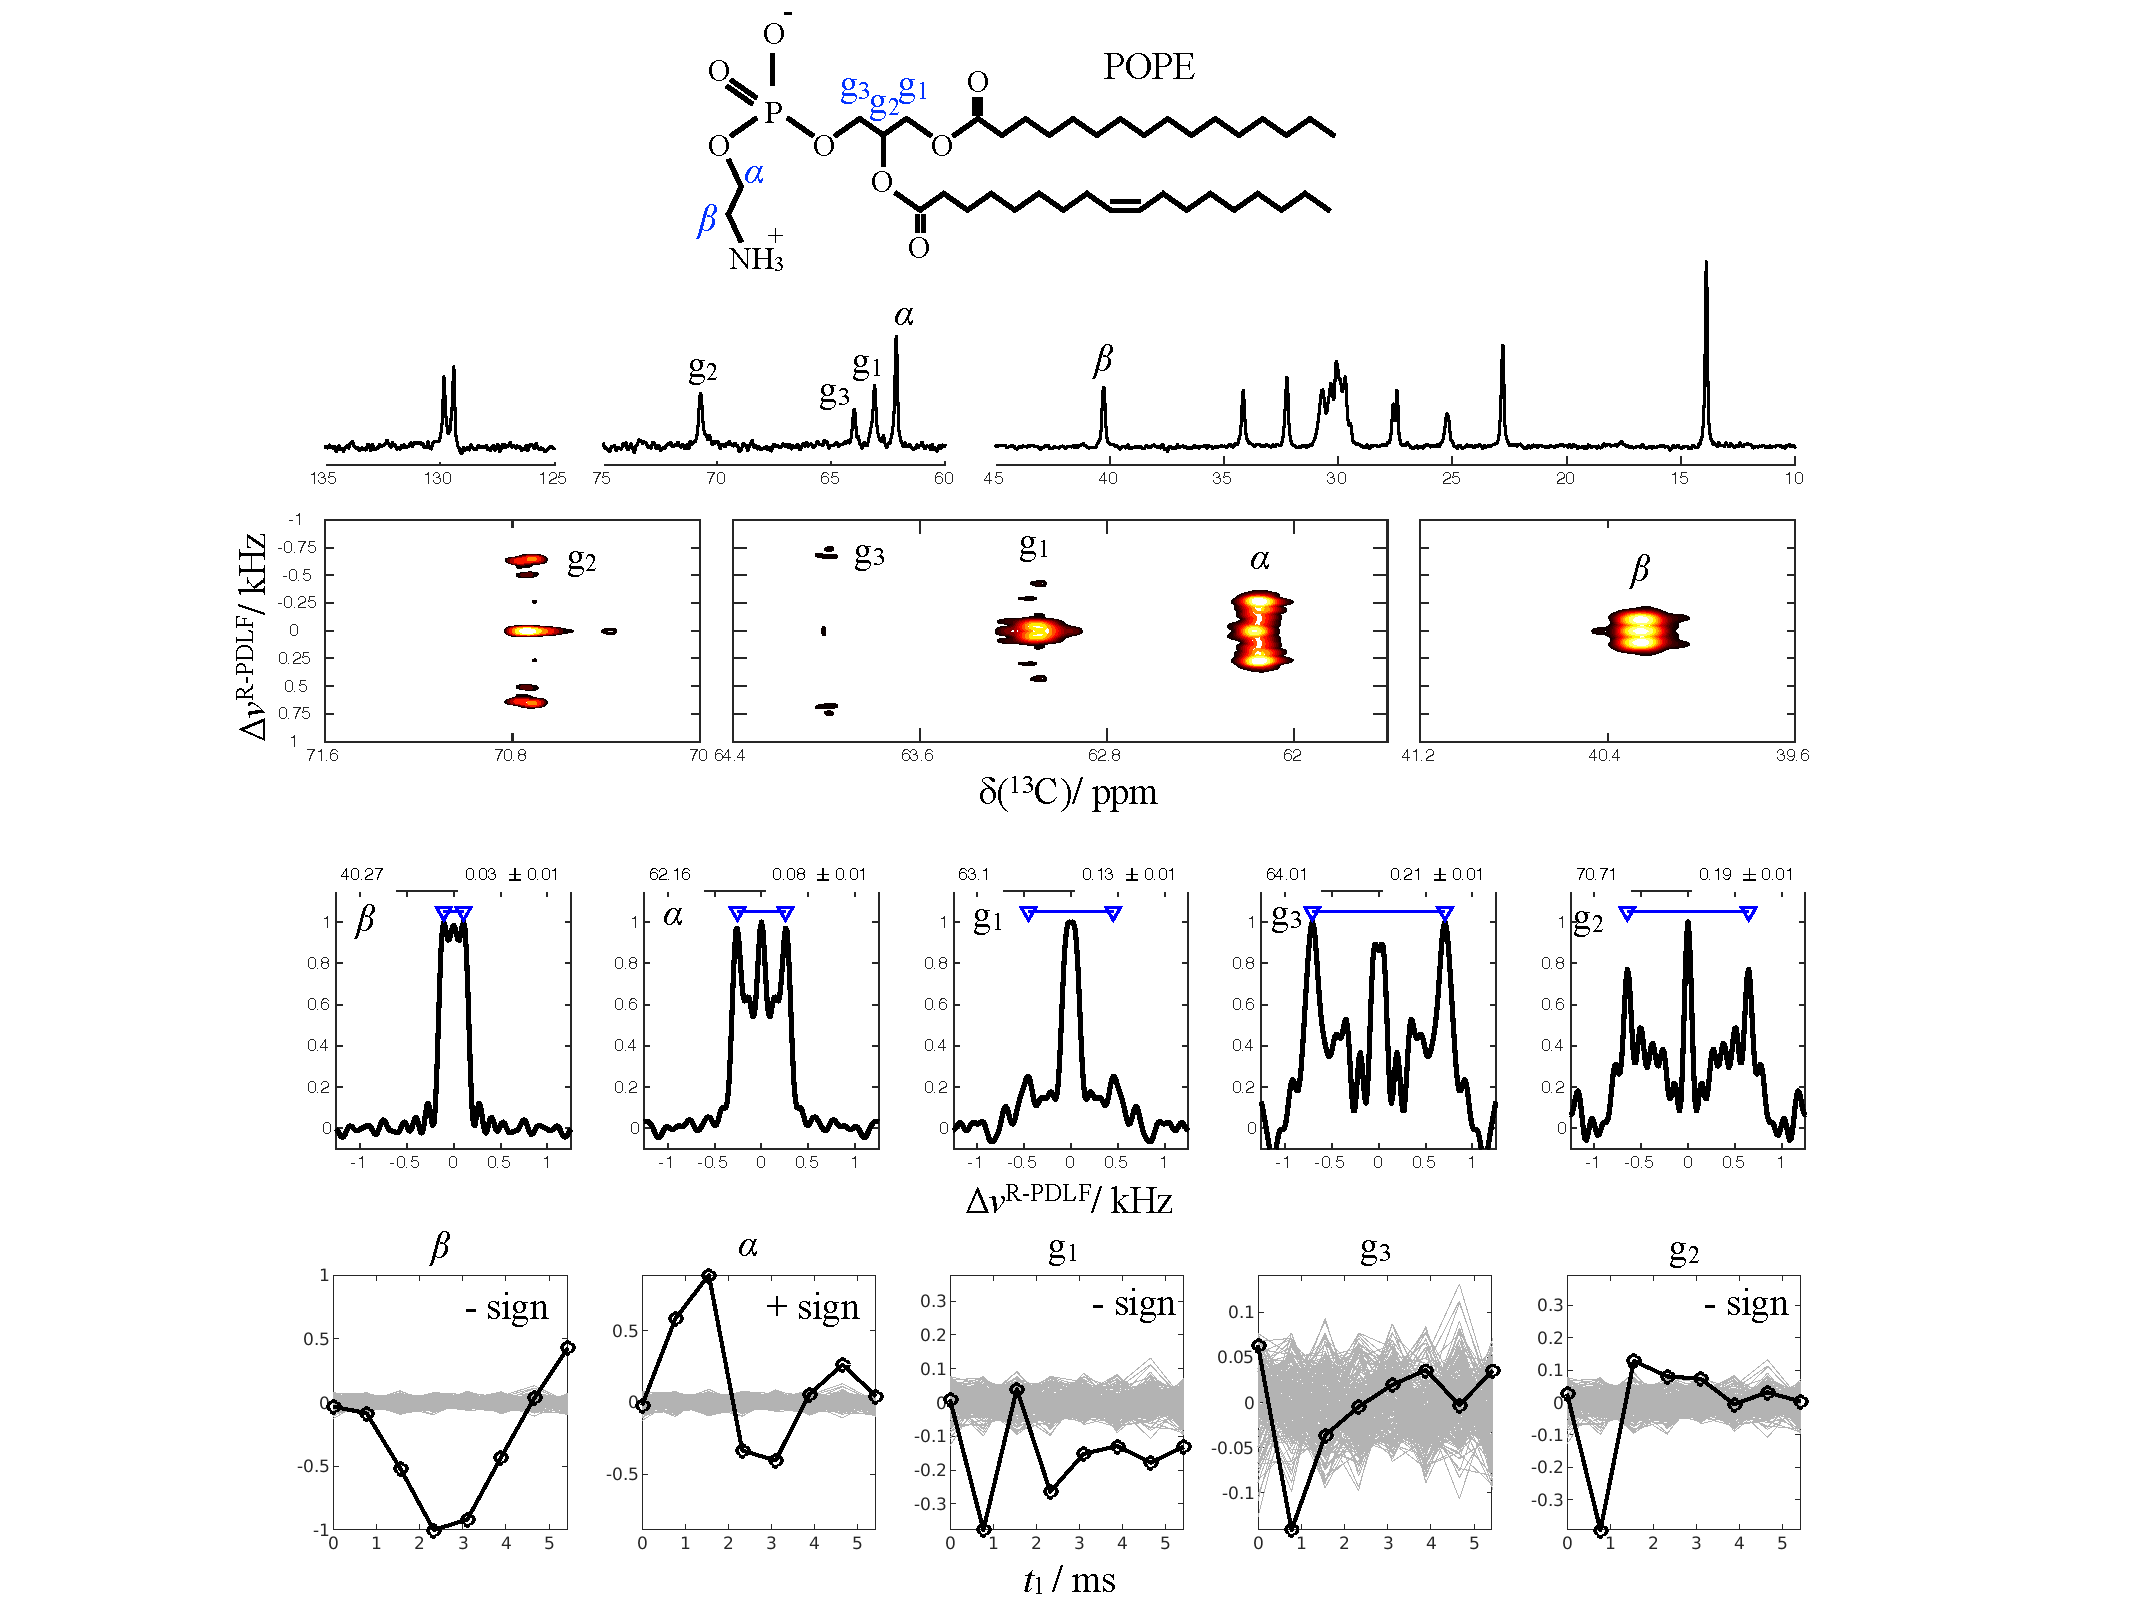
\includegraphics[width=\textwidth]{../Figs/POPEexperiment.pdf}
  \caption{\label{POPEspectra}
    (A) Chemical structure of POPE with the labeling of headgroup and glycerol backbone carbons.
    (B) INEPT spectra from POPE sample with the headgroup and glycerol backbone peaks labeled.
    (C) 2D R-PDLF spectra
    (D) Dipolar sliced from the  2D R-PDLF spectra with the resulting order parameters on top of figures.
    (E) Experimetal S-DROSS curves giving signs of the order parameters.
  }
  \todo{A, B etc. labels to be put in the figure.}
\end{figure}

\clearpage
\bibliography{refs.bib}

\end{document}
